\documentclass[12pt,a4paper]{article} 


\usepackage[spanish]{babel} 
\usepackage[utf8]{inputenc}
\usepackage[numbers,sort&compress]{natbib} 
\usepackage{graphicx} 
\usepackage{amsfonts}
\usepackage[left=2cm,right=2cm,top=2cm,bottom=2cm]{geometry}
\usepackage{listings}
\usepackage[usenames,dvipsnames]{color}



\title{Matemáticas Computacionales \\ Práctica 2: Estudio de una Base de Datos} 
\author{Arely Anahi Alvarado Solis \\ 1904628} 
\date{}

\begin{document}
\maketitle

\section{Introducción} \label{sec:intro}
En esta práctica se estudiara un base de datos con la estadística descriptiva básica. Se analizara los atributos, tipos de datos, indicadores básicos de una y de dos variables. Se muestran algunos de los primeros pasos para luego implementar un preprocesamiento de datos para luego utilizarla en alguna experimentación o trabajo a tratar.

\section{Base de Datos: cars}
Dada esta base de datos identificada como cars son los datos que dan la velocidad de los automóviles y las distancias que se toman para detenerse. Tomemos en cuenta que los datos que se registraron fueron en la década de 1920. Esto se implementa en \citep{data} y \citep{correlation}

\subsubsection{Descripción del conjunto de datos}
El datasets cars tiene 50 observaciones y aparte cuenta con 2 atributos que son:
\begin{enumerate}
       \item Velocidad ("mph": milla por hora)
       \item Distancia de frenado ("ft": pies)
\end{enumerate}

\subsection{Estadística descriptiva de una variable} \label{subsec:estadistdescrpuna}
Los datos de velocidad marca con un valor mínimo de 4.00, un máximo de 25.00, una mediana de 15.00 y media de 15.9; los datos de la distancia de frenado contiene un valor mínimo de 2.00, un valor máximo de 120.00, una mediana de 36.00 y una media de 42.98, esto se ve en la Figura (\ref{fig:densidad}).

\begin{figure}
\centering
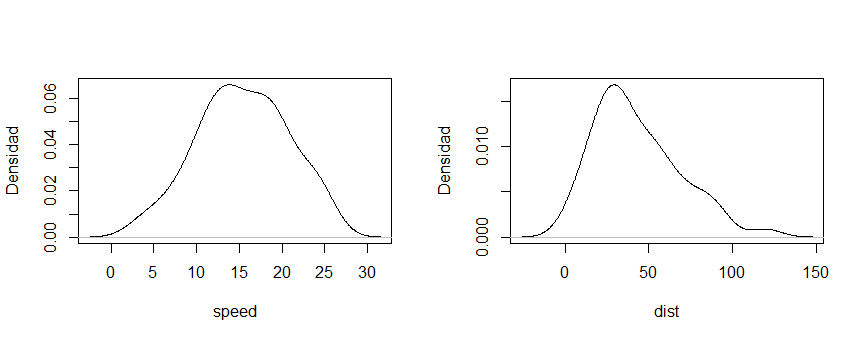
\includegraphics[scale=0.5]{densidad}
\caption{Gráfica de densidad de los atributos.}
\label{fig:densidad}
\end{figure} 

Con 12.00 sea el primer cuartil, el tercer cuartil de 19.00 y la mediana, que comentamos anteriormente, de 15.00, son datos de $velocidad$ y se ven en la Figura (\ref{fig:boxpSpeed}) ademas, se observa donde se encuentra el valor mínimo y máximo. 

\begin{figure}
\centering
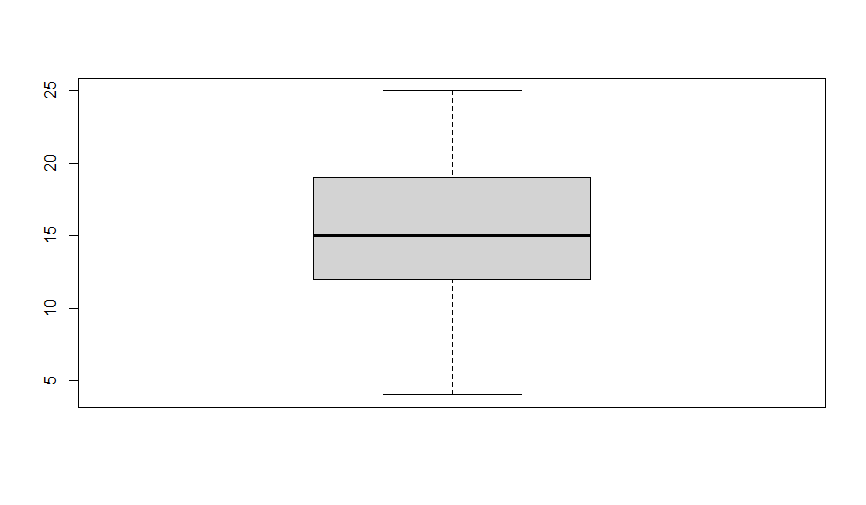
\includegraphics[scale=0.5]{boxplotSpeed}
\caption{Gráfica de caja bigotes de la velocidad.}
\label{fig:boxpSpeed}
\end{figure}

Aparte los datos de $distancia de frenado$, tenemos con el primer cuartil 26.00, el tercero con 56.00 y la mediana, que también comentamos anteriormente, de 36.00; esto se ve en la gráfica de la Figura (\ref{fig:boxpDist}) ademas, se ve donde se encuentra el valor mínimo y máximo.

\begin{figure}
\centering
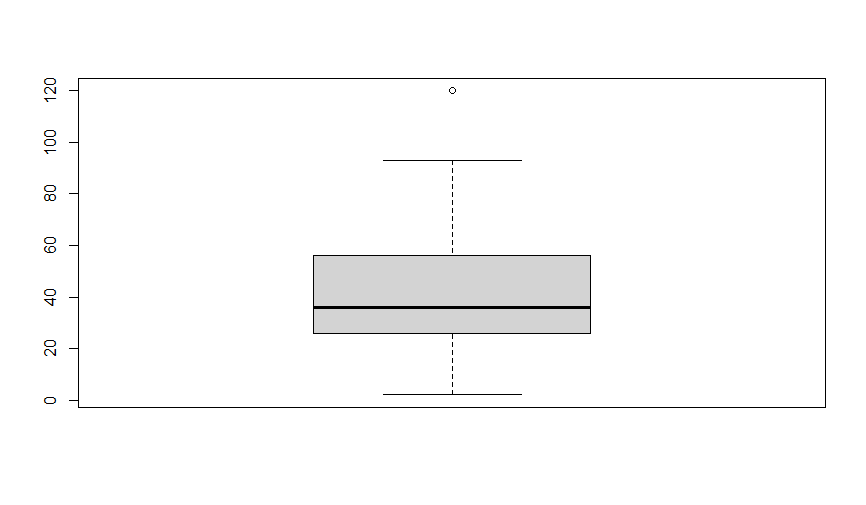
\includegraphics[scale=0.5]{boxplotDist}
\caption{Gráfica de caja bigotes de la distancia de frenado.}
\label{fig:boxpDist}
\end{figure}

\newpage
\subsection{Estadística descriptiva de dos variables} \label{subsec:estadistdescrpdos}

En la Figura (\ref{fig:correlations}) se muestra la correlación entre los únicos dos atributos utilizando el coeficiente de correlación de Pearson, donde se ve que dado los unicos dos atributos no hay mucho que decir entre estos, pues como va en un rango de [-1,1], se ve que ambos estan fuertemente correlacionados ya que ambos se acercan al 1 positivo.

\begin{figure}
\centering
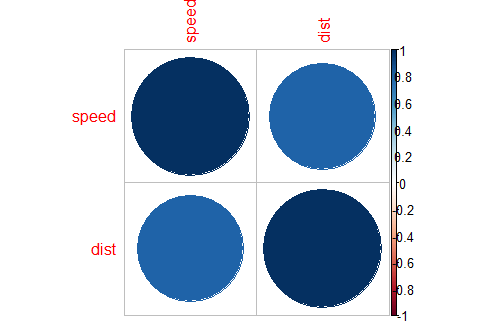
\includegraphics[scale=0.5]{correlations}
\caption{Gráfica de correlaciones entre los atributos.}
\label{fig:correlations}
\end{figure}

En las graficas de las Figuras (\ref{fig:scatterplot1}) y (\ref{fig:scatterplot2}) se ven los dos atributos correlacionados, donde se ve que indica una relación positiva entre ellas.

\begin{figure}
\centering
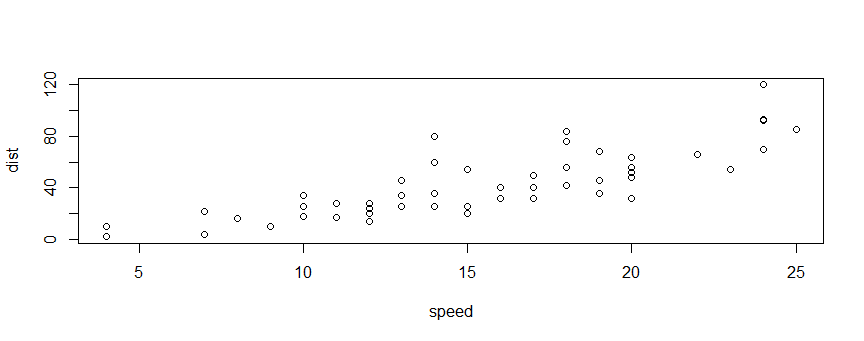
\includegraphics[scale=0.5]{scatterPlot}
\caption{Gráfica de dispersión 1 (scatterplot).}
\label{fig:scatterplot1}
\end{figure}

\begin{figure}
\centering
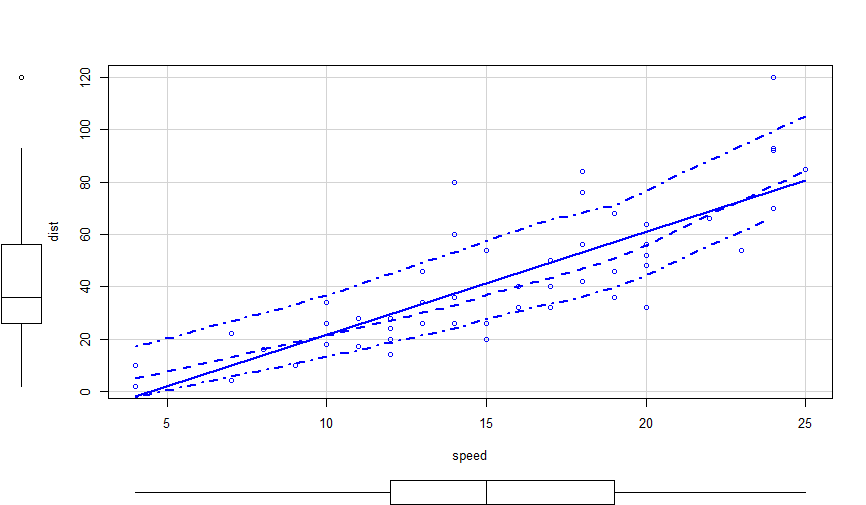
\includegraphics[scale=0.5]{ScatterPlot2}
\caption{Gráfica de dispersión 2 (scatterplot).}
\label{fig:scatterplot2}
\end{figure}

\newpage
Puede encontrar los códigos en el repositorio \citep{repositorio}

\bibliography{bibl}
\bibliographystyle{plainnat}


\end{document}